%%%%%%%%%%%%%%%%%%%%%%%%%%%%%%%%%%%%%%%%
% University/School Laboratory Report
% LaTeX Template
% Version 3.1 (25/3/14)
%
% This template has been downloaded from:
% http://www.LaTeXTemplates.com
%
% Original author:
% Linux and Unix Users Group at Virginia Tech Wiki 
% (https://vtluug.org/wiki/Example_LaTeX_chem_lab_report)
%
% License:
% CC BY-NC-SA 3.0 (http://creativecommons.org/licenses/by-nc-sa/3.0/)
%
%%%%%%%%%%%%%%%%%%%%%%%%%%%%%%%%%%%%%%%%%

%----------------------------------------------------------------------------------------
%   PACKAGES AND DOCUMENT CONFIGURATIONS
%----------------------------------------------------------------------------------------

\documentclass{article}

\usepackage[version=3]{mhchem} % Package for chemical equation typesetting
\usepackage{siunitx} % Provides the \SI{}{} and \si{} command for typesetting SI units
\usepackage{graphicx} % Required for the inclusion of images
\usepackage{natbib} % Required to change bibliography style to APA
\usepackage{amsmath} % Required for some math elements 
\usepackage{listings}
\usepackage{float}
\usepackage[center]{caption}
\usepackage{enumerate}
\usepackage{soul}
\usepackage{csquotes}

%\setlength\parindent{0pt} % Removes all indentation from paragraphs

%\renewcommand{\labelenumi}{\alph{enumi}.} % Make numbering in the enumerate environment by letter rather than number (e.g. section 6)

%\usepackage{times} % Uncomment to use the Times New Roman font

%----------------------------------------------------------------------------------------
%   DOCUMENT INFORMATION
%----------------------------------------------------------------------------------------

\date{\today} % Date for the report

\begin{document}
% Define document title and author
\title{Fourier Methods}
\author{Johnny Pribyl}
\markboth{Montana State University}{}
\maketitle

\begin{abstract}

    asdf
    
\end{abstract}



%----------------------------------------------------------------------------------------
%   SECTION 1
%----------------------------------------------------------------------------------------
\section{Introduction}

Almost every material has some degree of magnetism present. However, magnetic
forcs have a tendency to be quite weak (to the point of being largely
imperceptible). Unlike gravitational forces, electromagnetic forces can be
attractive or repulsive. Additionally, any time you place an object 
inside a magnetic field, the charges inside it tend to move around. 
Weasel's are funny, so let's pretend that we have a weasel sitting between a couple of magnets.

As the weasel's charges move around, they create \textit{another} magnetic field. 
Sometimes this second `induced' magnetic field is in the same direction as the original field, 
and other times it is in the opposite direction. I've never heard of an induced 
field that goes off in some random direction.. but magnets (and weasels) tend to have 
minds of their own, so maybe it's possible. At any rate, if the weasel's induced 
field is in the same direction as the original, we would call the weasel
Paramagnetic. If it is in the opposite direction, we would call the weasel
Diamagnetic.

In this lab, we examine the magnetic properties of several substances to figue
out how many charges like to move around and what direction they tend to move.

Just like last time, you can find all of my code at:
\begin{verbatim}
    jpribyl/cautious-palm-tree
\end{verbatim}

%----------------------------------------------------------------------------------------
%   SECTION 2
%----------------------------------------------------------------------------------------
\section{Objectives}

This lab has three main objectives. If you're not familiar with the methods and
procedures of this lab, then I would suggest reviewing the manual. It lives in:

\begin{verbatim}
lab2/lab_descrip/Foundational_Magnetic_Susceptibility_Manual.pdf
\end{verbatim}

\subsection{B Field Calibration}
Before we can start doing any kind of analysis on the data that we collected,
we had to calibrate the magnetic field between the magnets. Neodymium magnets
can be quite strong. We expected a result on the order of .5 Tesla. 

It is not possible (or at least not feasible) to measure the magnetic field
directly. Instead we measured the mass of the magnet. Then, we placed a copper
sheet between the magnet and ran a strong current through it. We measured the
change in mass of the magnet and used this equation to calculate B:
$$\vec{F} = \frac{A \chi_m (B_{b}^{2} - B_{t}^{2})}{2 \mu_0}$$
We found that keeping the copper sheet over the top of the magnet has a
negligible effect upon the mass of the system. It did not register at all on
the Guoy Balance. So, we were able to conclude that $B_t$ is zero and solve for
$B_b$:

$$B_b = \frac{2 \mu_0 (m_1 - m_0) g}{A \chi_m}$$
Where $m_1$ is the mass of the system with the current running through it and
$m_0$ is the mass of the magnet by itself. Note that when there is no mass
change, the magnetic field vanishes.

The data that we collected is available in data/magnetic.xlsx 
and my lab notebook, so I will not recopy it here. But, here is what it looks
like:

\begin{figure}[H]
        % Center the figure.
        \begin{center}
        % Include the eps file, scale it such that it's width equals the column width. You can also put width=8cm for example...
        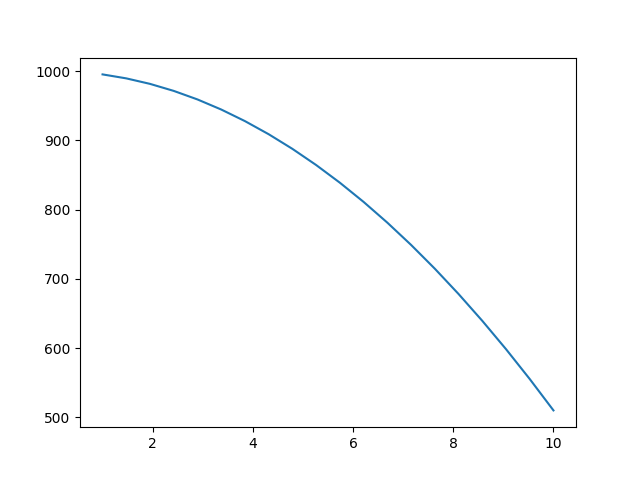
\includegraphics[width=8cm, height=6cm]{/home/johnny/kod/py/bin/venv/py3/phx444/labs/lab2/figures/figure1.png}
        % Create a subtitle for the figure.
        \caption{Plotting the Measured values for Magnetic Field}
        % Define the label of the figure. It's good to use `fig:title', so you know that the label belongs to a figure.
        \label{fig:fig_1}
        \end{center}
\end{figure}
I chose to read my data into python as a Pandas DataFrame. In my experience,
pandas is just about the best library to work with heterogeneous data. It's
even able to read an excel file:
\begin{center}
\begin{minipage}[t]{.75\textwidth}
\begin{lstlisting}[frame=tlrb]
xl = pd.ExcelFile(`data/magnetic.xlsx')
df = xl.parse(`Sheet1')
\end{lstlisting}
\end{minipage}
\end{center}
After that, I dropped the non-existent entries off the bottom of the DataFrame
because they're problematic for model fitting. Then, I used the uncerainties
package and a lambda function to propagate error through all of our mass and 
current measurements. I'm not going to copy all of the code here, but the
general syntax follows this form:
\begin{center}
\begin{minipage}[t]{.75\textwidth}
\begin{lstlisting}[frame=tlrb]
<Measurement>= \
    df[<Measurement>].dropna().apply(
        lambda x: ufloat(x, <error>)
    )
\end{lstlisting}
\end{minipage}
\end{center}
Next, for the current menasurements, I looked up the specs for
Keithley's model 2000 6 1/2 digit multimeter. I stared at them for a while.
Then I pestered Brian for a while. Then I stared at the specs some more. Eventually, I
pestered Brian enough that he showed how to read the table. In our case, the current 
has an uncertainty of:
$$(1000 \times I + 3 \times 15) \times 10^{-6}$$
In python, we are able to make use of the pandas data structure and
uncertainties library to propagate this:
\begin{verbatim}
current_error = \
    1000 * df[`current'].dropna() * 10 ** -6 + 3 * 15 * 10**-6

b_cal_current = \
    pd.Series(uarray(df[`current'].dropna(), current_error))
\end{verbatim}
Notice that I have to explicitly turn the result back into a
pandas object. The uarray() method returns a NumPy Array. It would be totally
fine to leave the result as a NumPy object, but syntactically NumPy is slightly
different and Pandas, so it's beneficial to have all objects be the same type.

I was able to fit the curve using the same method as in the data
analysis lab. Specifically, I assumed linearity and fit it with:

\begin{center}
\begin{minipage}[t]{.75\textwidth}
\begin{lstlisting}[frame=tlrb]
def lin_fit(x, a, b):
    return a*x + b

popt, pcov = curve_fit(
                lin_fit, 
                current_values, 
                b_cal_values
            )

b_fit = lin_fit(
    current_values, 
    *popt
)
\end{lstlisting}
\end{minipage}
\end{center}

We learned last lab that residuals are a pretty decent sanity check on the
accuracy of data and models. So let's go ahead and plot the residuals from this
fit:

\begin{center}
\begin{minipage}[t]{.75\textwidth}
\begin{lstlisting}[frame=tlrb]
r_i = b_cal_values - b_fit

plt.errorbar(
    current_values,
    r_i,
    yerr=b_cal_error,
    fmt='o')
\end{lstlisting}
\end{minipage}
\end{center}

And showing this plot, we find that the residuals are actually quite
reasonable. They are clustered around zero and their error bars are easily
visible. Notice that the size of the error bars around zero is quite large.
This makes sense because the current error ought to be similar in magnitude, but
its fractional error will increase:

\begin{figure}[H]
        % Center the figure.
        \begin{center}
        % Include the eps file, scale it such that it's width equals the column width. You can also put width=8cm for example...
        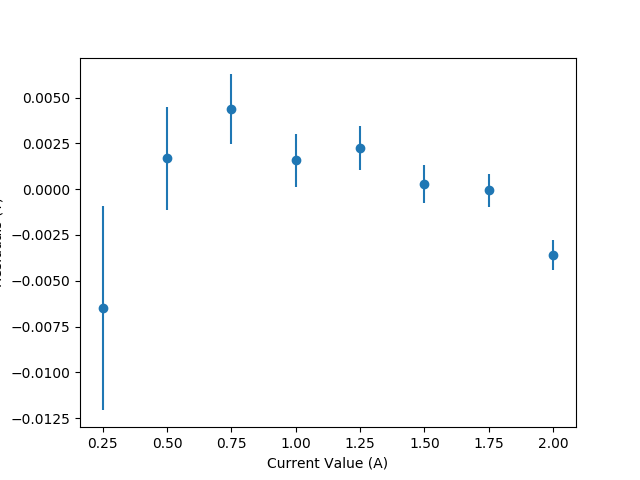
\includegraphics[width=8cm,
        height=6cm]{/home/johnny/kod/py/bin/venv/py3/phx444/labs/lab2/figures/figure1b.png}
        % Create a subtitle for the figure.
        \caption{Plotting the residuals as a sanity check}
        % Define the label of the figure. It's good to use `fig:title', so you know that the label belongs to a figure.
        \label{fig:fig_2}
        \end{center}
\end{figure}


\subsection{Magnetic Susceptibility of Samples}
Now, hopefully I've convinced you that the environment between our magnets
houses a magnetic field that is approximately .4 Teslas. If I haven't
convinced you yet, try this:

\begin{center}
\begin{minipage}[t]{.75\textwidth}
\begin{lstlisting}[frame=tlrb]
def understand(paper, confused=True):
    if confused:
        read(section_1)
        read(section_2)
        understand(paper)

    return 
\end{lstlisting}
\end{minipage}
\end{center}

Moving right along, We massed all our samples using the Guoy balance. Then, we
did some math to determine how much of our sample was empty space and how much
was really the substance in question. For example, if you have a vial full of pebbles, then
a good bit of the vial is actually just air. The actual area is given by:
$$A = (w\times l)(\% real)$$
Where \% real is: 
$$\frac{ m_{measured}}{ m_{theoretical}}$$
And, for a substance of known density $\rho$, theoretical mass is:
$$volume \times \rho$$
Putting all of that together with the equation that we derived in lecture, we
find the magnetic susceptibilty with:
$$\chi_m = \frac{2 \times \mu_0 \times g (m_1 - m_0)}{A B^2}$$
As before, $m_1$ refers to the mass of the magnet apparatus with the sample
sitting in between the magnet and $m_0$ is the mass of the magnet without a
sample in between it. 

One peculiarity that I had not considered prior to doing my data analysis was
the possibility of getting a value larger than 1 for \% real. This does not
physically make sense (because our samples were not pressurized). For most of the
samples, this was not an issue. 

However, for the two wire samples, things got a little
interesting. The wires were too small for us to measure very accurately which
led us to accumulate immensely large errors.  After thinking on the issue for a
while, eventually I decided to accept the measurements on these wires that are
provided in the lab to be exact. I also decided to refuse negatve percentages
and cap the maximum \% real at 1. 

In python, we can impose reaonability on percentages with: 

\begin{center}
\begin{minipage}[t]{.75\textwidth}
\begin{lstlisting}[frame=tlrb]
percent_real = (real_mass / theory_mass)

percent_real.apply(
    lambda x: ufloat(min(abs(x.n), 1), x.s)
)
\end{lstlisting}
\end{minipage}
\end{center}

Then, we can drop the error from cobalt:

\begin{center}
\begin{minipage}[t]{.75\textwidth}
\begin{lstlisting}[frame=tlrb]
area[4] = area[4].n
percent_real[4] = percent_real[4].n
\end{lstlisting}
\end{minipage}
\end{center}

And now we're off to the races! Doing all the math things and putting them in a
table thing that compares measurements and uncertainties to accepted $\chi_m$
values, we see that most of our results are actually quite good:

\begin{figure}[H]
        % Center the figure.
        \begin{center}
        % Include the eps file, scale it such that it's width equals the column width. You can also put width=8cm for example...
        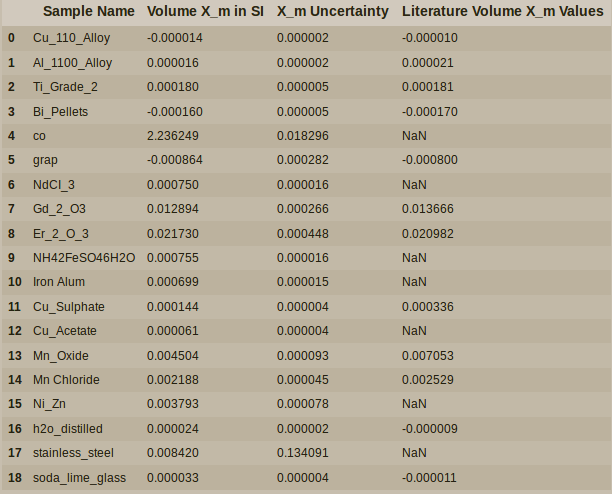
\includegraphics[width=10cm, height=10cm]{/home/johnny/kod/py/bin/venv/py3/phx444/labs/lab2/figures/tablefigure.png}
        % Create a subtitle for the figure.
        \caption{A table with our results}
        % Define the label of the figure. It's good to use 'fig:title', so you know that the label belongs to a figure.
        \label{fig:fig_4}
        \end{center}
\end{figure}

However, there were a couple of surprises! I was shocked at the lack
of literature data for comparison. Most of the data that I \textit{was} able to
find was not available in SI units. The conversion from $\chi_{molar}$ in cgs
to volume $\chi_m$ in SI must be done in 2 steps. First, you convert to volume
$\chi_m$ in cgs and second, you multiply by the conversion factor of $4 \pi$.
These units are very picky and I still don't fully understand why.

Also, it seems as though something went a bit wrong when we prepared our own
samples! While the majority of our data falls within 3 $\sigma$ of the
literature values, we did not even get the correct sign for Water or Soda Lime
Glass. Maybe we should have been a bit more suspicious of the bottle labeled
``distilled water."



%----------------------------------------------------------------------------------------
%   SECTION 4
%----------------------------------------------------------------------------------------
\section{Questions}
\subsection{Units Of $\chi_m$}

There are a few common units for $\chi_m$ because there are a few different
flavors of susceptibility. In class we discussed that Volume $\chi_m$ is
actually unitless. This is true in both cgs and SI - however, there \textit{is
    still a conversion factor between them}. I find that pretty strange, but I
learned to stop questioning units when I started measuring the mass of the sun
in kilometers.

You might also encounter a molar $\chi_m$. In CGS this has units of
$\frac{cm^3}{mol}$ but Brian told us that in SI, molar $\chi_m$ has units of
$\frac{kg}{mol}$. That's pretty neat, but Wikipedia disagrees with Brian.
Wikipedia says that molar $\chi_m$ has units of $\frac{m^3}{mol}$ in SI.

The last type of $\chi_m$ that Brian mentioned is mass $\chi_m$. In SI this has
units of $\frac{m^3}{kg}$ while in cgs it is $\frac{cm^3}{g}$.

\subsection{Compare Results to Literature Values}
It's tough to compare our results to literature values, because quite a few of
the literature values don't exist. And, when they do exist they're in the wrong
units. So, in order to do any comparison I had to start by collecting as many
literature values for $\chi_m$ as I could find. I converted the cgs values of
$\chi_{mol}$ into volume $\chi_m$ in SI like this:
$$\chi_{sivol} = 4 \pi\frac{\chi_{cgsmol}}{M_{cgs} / \rho_{cgs}} $$
Where M is the molar mass. If we plot this with the literature values along the
x axis and measure values along the y axis, we would expect the line y = x to
intersect most of them. I went one step further and ran a linear fit on our
data points using the same curve\_fit method that I describe in section 2.1.
Plotting the results, we see that, overall, our data agrees with the
literature:


\begin{figure}[H]
        % Center the figure.
        \begin{center}
        % Include the eps file, scale it such that it's width equals the column width. You can also put width=8cm for example...
        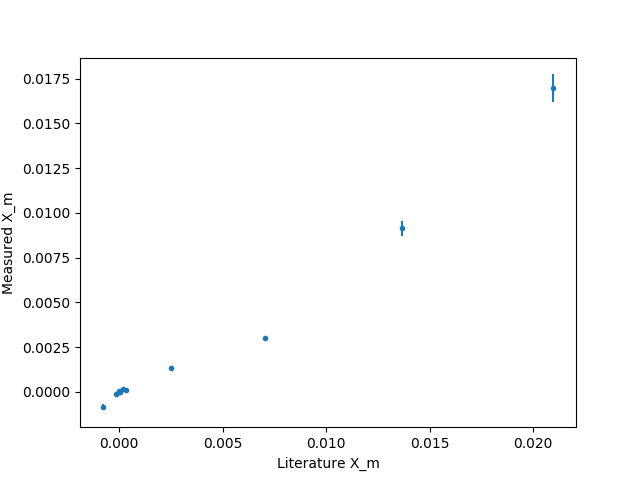
\includegraphics[width=8cm, height=6cm]{/home/johnny/kod/py/bin/venv/py3/phx444/labs/lab2/figures/figure8.png}
        % Create a subtitle for the figure.
        \caption{Plotting accepted values for $\chi_m$ against our measurements}
        % Define the label of the figure. It's good to use 'fig:title', so you know that the label belongs to a figure.
        \label{fig:fig_5}
        \end{center}
\end{figure}

\subsection{Levitation!!}
Brian gave this one away. I'm going to go out on a limb here and say that
pyrolitic graphite might work, just maybe. Here's what it looks like:


\begin{figure}[H]
        % Center the figure.
        \begin{center}
        % Include the eps file, scale it such that it's width equals the column width. You can also put width=8cm for example...
        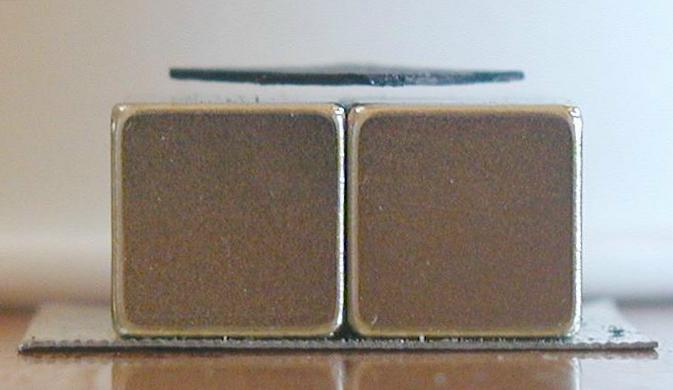
\includegraphics[width=8cm, height=6cm]{/home/johnny/kod/py/bin/venv/py3/phx444/labs/lab2/figures/levitation.jpg}
        % Create a subtitle for the figure.
        \caption{Photo credits to the kind folks over at: http://sci-toys.com}
        % Define the label of the figure. It's good to use 'fig:title', so you know that the label belongs to a figure.
        \label{fig:fig_6}
        \end{center}
\end{figure}

Sci-toys has a really great explanation of the phenomenon. It's worth reading
if you like science. Here's an excerpt that will (hopefully) get you excited
enough to open up a browser:
\begin{quotation}

 ``We can do that by using four magnets. The poles of the magnets push on the
 diamagnetic material more strongly than other parts of the magnet. With four
 magnets, the four edges of the square of pyrolytic graphite will be pushed
 away from the four poles."

 - sci-toys.com

\end{quotation}

\section{Conclusion and Sources of Error}

I must say, I'm pretty impressed with our results. I fully expected them to
wildly disagree with the accepted values of $\chi_m$. During the experiment, we
noticed that the instruments were incredibly sensitive. Things like leaning on
the table, or rotating the balance made noticeable impacts upon results. We
also noticed that the scale's calibration had a tendency to walk. And, paralax
made it quite difficult to ensure that the bottom of our samples was precisely
in the middle of the magnetic field. 

The only significant source of error seemed to occur during the preparation of
our own samples. It's possible that the vials were not adequately cleaned. It's
even possible that the samples we prepared were not quite exactly what we
thought they were. Lastly, it's possible that the literature values for
$\chi_m$ are wrong.

If I were to do this experiment again, I would be more careful to monitor the
walking of the scale's calibration and more careful while preparing my own
samples.

\end{document}
